\subsection{Overview}
In this section we discuss the process that has been conceived and applied to evaluate the
performance of \emph{CROSSSIM} in comparison some baselines. As stated before we opted for \emph{MUDABLUE} and
\emph{CLAN}. The rationale behind the selection of these approaches is that they are well-established algorithms.

\subsection{Dataset}

To serve as input for the evaluation, it is necessary to populate a dataset that meets the requirements by all four approaches. By MUDABlue and CLAN, there are no specific requirements since both metrics rely solely on source code to function. However, for CrossSim, we consider only projects that satisfy certain criteria. In particular, we collected projects that meet the following requirements:

\begin{itemize}
	\item Being GitHub Java projects; 
	\item Providing the specification of their dependencies by means of "code.xml" or ".gradle" files.;
	\item Including at least $9$ dependencies. A project with no or little information about dependencies may adversely affect the performance of CrossSim; 
	\item Having the "README.md" file available; 
\end{itemize}

Furthermore, we realized that the final outcomes of a similarity algorithm are to be validated by human beings, and in case the projects are irrelevant by their very nature, the perception given by human evaluators would also be \emph{dissimilar} in the end. This is valueless for the evaluation of similarity. Thus, to facilitate the analysis, instead of crawling projects in a random manner, we first observed projects in some specific categories (e.g. PDF processors, JSON parsers, Object Relational Mapping projects, and Spring MVC related tools). Once a certain number of projects for each category had been obtained, we also started collecting randomly to get projects from various categories.

Using the GitHub API\footnote{GitHub API: \url{https://developer.github.com/v3/}}, we crawled projects to provide input for the evaluation. Though the number of projects that fulfill the requirements of a single approach, i.e. either RepoPal or CrossSim, is high, the number of projects that meet the requirements of both approaches is considerably lower. For example, a project contains both "pom.xml" and "README.md", albeit having only $5$ dependencies, does not meet the constraints and must be discarded. The crawling is time consuming as for each project, at least $6$ queries must be sent to get the relevant data. GitHub already sets a rate limit for an ordinary account\footnote{GitHub Rate Limit: \url{https://developer.github.com/v3/rate_limit/}}, with a total number of $5,000$ API calls per hour being allowed. And for the search operation, the rate is limited to $30$ queries per minute. Due to these reasons, we ended up getting a dataset of $580$ projects that are eligible for the evaluation. The dataset we collected and the CrossSim tool are already published online for public usage \cite{CROSSSIM-DATA}.

%\subsubsection{Data collection} \label{sec:DataCollection}

%In addition, to facilitate the evaluation of similarity and clustering techniques, instead of crawling projects in a random manner, we first observed projects in some specific categories. We suppose that the evaluation might lead to a cumbersome process if we consider arbitrary projects which are generally not related. The final outcomes of a similarity algorithm need to be validated by human beings, and given that the projects are irrelevant by their very nature, the perception given by human evaluators would also be \emph{dissimilar} in the end, and this is valueless for the evaluation of similarity. 


Further than collecting projects for each category, we also started collecting random projects. These projects serve as a means to test the stability of the algorithms. If the algorithms work well, they will not perceive newly added random projects as similar to projects of some other specific categories. To this end, the categories and their corresponding cardinality to be studied in our evaluation are listed in Table \ref{tab:Categories}. This is an approximate classification since a project might belong to more than one category.

\begin{table}[h!]
	\small
	\centering
	\begin{tabular}{|p{0.80cm}|p{5.00cm}|p{2.30cm}|}  \hline
		{\bf No.} & {\bf Name} & {\bf \# of Projects} \\  \hline
		1 & SPARQL, RDF, Jena Apache & 21 \\  \hline
		2 & PDF Processor & 8  \\  \hline
		3 & Selenium Web Test & 26  \\  \hline
		4 & ORM & 13  \\  \hline
		5 & Spring MVC & 51  \\  \hline
		6 & Music Player & 25  \\  \hline
		7 & Boilerplate & 38  \\  \hline
		8 & Elastic Search & 55  \\  \hline
		9 & Hadoop, MapReduce & 52  \\  \hline
		10 & JSON & 20  \\  \hline
		11 & Miscellaneous Categories & 271  \\  \hline
	\end{tabular}
	\caption[List of software categories]{List of software categories}
	\label{tab:Categories}
\end{table}

As can be seen in Table \ref{tab:Categories}, among $580$ considered projects, $309$ of them belong to some specific categories, such as \emph{SPARQL, RDF, Jena Apache}, \emph{Selenium Test}, \emph{Elastic Search}, \emph{Spring MVC}, etc. The other $271$ projects being selected randomly belong to \emph{Miscellaneous Categories}. These categories disperse in several domains and sometimes it happens that there is only one project in a category. %For the sake of clarity, we do not introduce the list of the categories in this deliverable.

%The random projects are used as a means to.
%From the dataset, a graph is built using the relationships in Section~\ref{sec:GraphRepresentation}. %There, nodes are either users, dependencies or projects and each is encoded using a unique number across the whole graph. Edges represent the corresponding relationships between users and projects or between dependencies and projects. 


%\paragraph{\textbf{Application of RepoPal and CrossSim}}
%\noindent\emph{\textbf{Application of RepoPal and CrossSim}}

\newpage
\subsection{User Study}
We involved a group of $15$ people software developers who have at least 5 years of experience in the user study. To get information about the participants related to their programming experience, we sent them a questionnaire similar to the one presented in \cite{McMillan:2012:DSS:2337223.2337267}.%\footnote{\url{http://www.cs.wm.edu/semeru/clan/CaseStudyMaterials.zip}}. 
According to the survey, we found out that most developers use StackOverflow to search for code.

\begin{table*}[h!]
	\centering
	%	\vspace{-.3cm}\\	
	\begin{tabular}{|p{2.4cm}|p{8.0cm}|p{1.0cm}|}  \hline
		{\bf Scale} & {\bf Description} & {\bf Score} \\  \hline
		Dissimilar & The functionalities of the retrieved project are completely different from those of the query project & 1 \\ \hline
		Neutral & The query and the retrieved projects share a few functionalities in common & 2 \\ \hline
		Similar & The two projects share a large number of tasks and functionalities in common & 3 \\ \hline
		Highly similar & The two projects share many tasks and functionalities in common and can be considered the same & 4 \\ \hline
	\end{tabular}
	%	\vspace{.1cm}	
	%	\vspace{-.2cm}
	\caption[Similarity scales]{Similarity scales}
	\label{tab:Scales}
\end{table*}

By the user study, in order to have a fair evaluation, for each query we mixed and shuffled the top-$5$ results generated from the computation by all similarity metrics in a single file and present them to the evaluators. This mimics a \emph{taste test} where users are asked to evaluate a product, (e.g. food or drink, without having a priori knowledge about what is being addressed \cite{Ghose2001},\cite{doi:10.1108/13522750810879048}). This aims at eliminating any bias or prejudice against a specific similarity metric. In particular, given a query, a user study is performed to evaluate the similarity between the query and the corresponding retrieved projects. The participants are asked to label the similarity for each pair of projects \emph{(, $<$\textit{query, retrieved project}$>$)}with regards to their application domains and functionalities using the scales listed in Table \ref{tab:Scales} \cite{McMillan:2012:DSS:2337223.2337267}. For example, an OSS project $p_{1}$ that performs the sending of files across a TCP/IP network is somehow similar to an OSS project $p_{2}$ that exchanges text messages between two users, \emph{i.e. $Score(p_{1},p_{2})=3$}. However an OSS project $p_{3}$ with the functionalities of a pure text editor is dissimilar to both $p_{1}$ and $p_{2}$, \emph{i.e. $Score(p_{1},p_{2})=Score(p_{1},p_{3})=1$}. Given a query, a retrieved project is considered as a \emph{false positive} if its similarity to the query is labeled as \emph{Dissimilar} ($1$) or \emph{Neutral} ($2$). In contrast, \emph{true positives} are those retrieved projects that have a score of $3$ or $4$, \emph{i.e. \emph{Similar} of \emph{Highly similar}}. A good similarity metric should produce as much true positives as possible.







\subsubsection{Calculation of metrics}

To evaluate the outcomes of the algorithms with respect to the user study, the following metrics have been considered as typically done in related work \cite{Lo:2012:DSA:2473496.2473616,McMillan:2012:DSS:2337223.2337267,10.1109/SANER.2017.7884605}:

\begin{itemize}
	\item \textit{Success rate}: if at least one of the top-5 retrieved projects is labelled \emph{Similar} or \emph{Highly similar}, the query is considered to be successful. {\em Success rate} is the ratio of successful queries to the total number of queries;
	\item \textit{Confidence}: Given a pair of $<$\textit{query, retrieved project}$>$ the confidence of an evaluator is the score she assigns to the similarity between the projects;
	\item \textit{Precision}: The precision for each query is the proportion of projects in the top-5 list that are labelled as \emph{Similar} or \emph{Highly similar} by humans. 
\end{itemize}

Further than the previous metrics, we introduce an additional one to measure the ranking produced by the similarity tools. For a query, a similarity tool is deemed to be good if all top-5 retrieved projects are relevant. In case there are false positives, i.e. those that are labeled \emph{Dissimilar} and \emph{Neutral}, it is expected that these will be ranked lower than the true positives. In case an irrelevant project has a higher rank than that of a relevant project, we suppose that the similarity tool is generating an improper recommendation. The \emph{Ranking} metric presented below is a means to evaluate whether a similarity metric produces properly ranked recommendations. 

\newpage
\subsection{Evaluation Results}
To study the performance of the metrics in detecting similar projects for the set of queries, the following research questions are considered:

\newcommand{\rqfirst}{RQ$_1$: Which similarity metric yields a better performance in terms of Success rate, and Precision?}\textit{\textbf{\rqfirst}} %: RepoPal or \CrossSim

By this question, we study the performance of different approaches.

\begin{figure}[H]
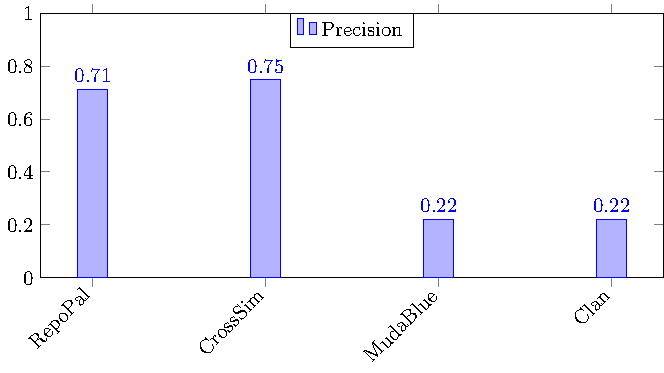
\includegraphics[width=10cm,height=15cm,keepaspectratio]{images/Precision.pdf}
\centering
\caption{Precision Comparison}
\label{fig:PrecisionC}
\end{figure}

Experimental results suggests that CrossSim approach overperforms all the other approaches, in particular Clan and MudaBlue.
Repopal got a good score, this means that is still a valid choice for similarity in the OSS environment.
The precision,as the figure~\ref{fig:PrecisionC} depicts, shows that CrossSim and Repopal got a score \emph{greater than 70\%}.
Clan and MudaBlue instead, reported a very low score, \emph{about 20\%}, on 10 queries evaluted, just 2 got a score \emph{$\geq3$}.

\begin{figure}[H]
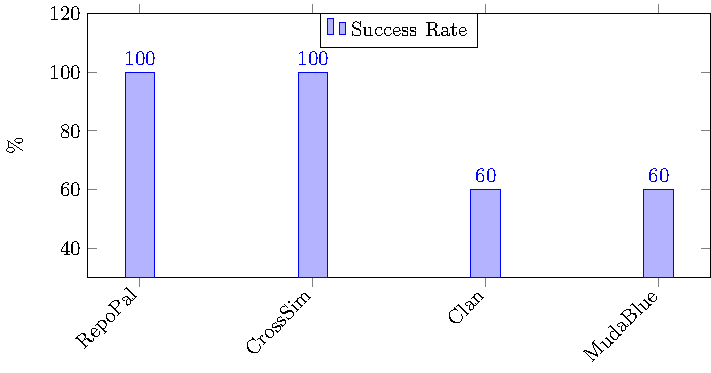
\includegraphics[width=10cm,height=15cm,keepaspectratio]{images/SuccessRate.pdf}
\centering
\caption{Success Rate Comparison}
\label{fig:SuccessC}
\end{figure}

Concerning the success rate, the results of CrossSim and Repopal are quite impressive, about \emph{100\%} of queries got score high, the situation is lower for Clan and MudaBlue that achieved just the \emph{60\%} of the queries. In order to calculate this values, we counted for each query how many votes were \emph{$\geq3$} divided then by 25, which is the number of queries.


\begin{figure}[H]
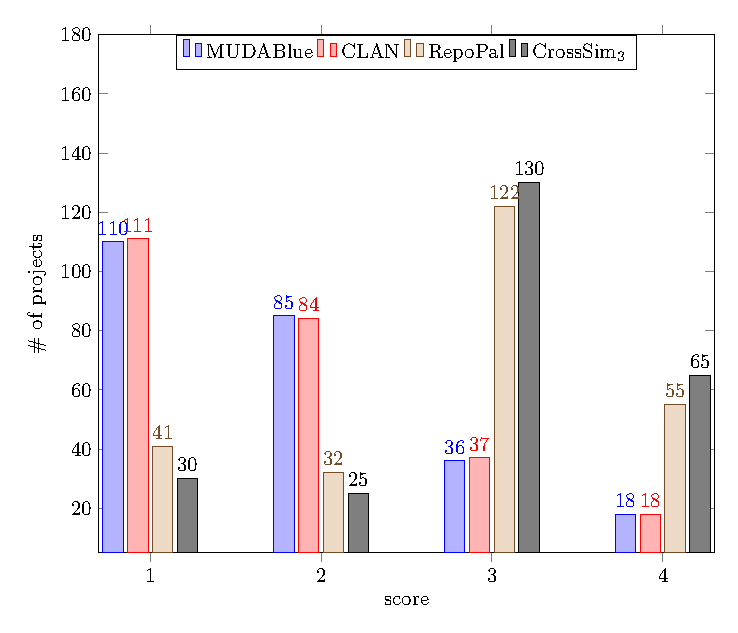
\includegraphics[width=10cm,height=15cm,keepaspectratio]{images/Confidence.pdf}
\centering
\caption{Confidence Comparison}
\label{fig:ConfidenceC}
\end{figure}

The confidence confirms what stated so far, the mojority of the votes for MudaBlue and Clan are between 1 and 2,that is, users evaluated as dissimilar most of the projects. For CrossSim the result is quite more nice, with 130 rank 3 votes and 60 rank 4 votes, so more than half results are good. Repopal also got a good evaluation, close to CrossSim but a bit lower.

\newcommand{\rqsecond}{RQ$_2$: Which similarity metric is more efficient?}\textit{\textbf{\rqsecond}} 

An important factor for a similarity metric is the ability to compute within an acceptable amount of time.

\begin{figure}[H]
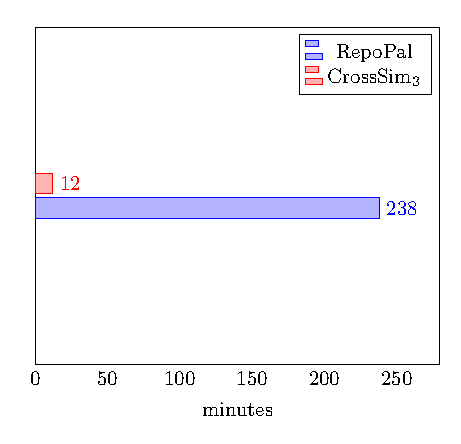
\includegraphics[width=8cm,height=13cm,keepaspectratio]{images/ExecutionTime.pdf}
\centering
\caption{Execution Time Comparison}
\label{fig:LabelC}
\end{figure}

\subsection{Threats to Validity}\label{sec:threatsValidity}

In this section, we investigate the threats that may affect the validity of the experiments as well as how we have tried to minimize them. In particular, we focus on the following threats to validity as discussed below. %internal and external 

\textit{\textbf{Internal validity}}  concerns any confounding factor that could influence our results.  We attempted to avoid any bias in the evaluation and assessment
phases: (\emph{i}) by involving three participants in the user study. In particular, the labeling results by one user were then double-checked by other two users to make sure that the outcomes were sound; (\emph{ii}) by completely automating the evaluation of the defined metrics without any manual intervention. Indeed, the implemented tools could be defective. To contrast and mitigate this threat, we have run several manual assessments and counter-checks.

\textit{\textbf{External validity}}  refers to the generalizability of obtained results and findings. Concerning the generalizability of our approach, we were able to consider a dataset of $580$ projects, due to the fact that the number of projects that meet the requirements of both RepoPal and CrossSim is low and thus required a prolonged crawling. During the data collection, we crawled both projects in some specific categories as well as random projects. The random projects served as a means to test the generalizability of our algorithm. If the algorithm works well, it will not perceive newly added random projects as similar to projects of the specific categories.

\textit{\textbf{Reliable validity}}  is related to the reproducibility of our experiments. To allow anyone to seamlessly replicate the evaluation, we made available the source code implementation of MUDABlue, CLAN, RepoPal, and CrossSim as also the dataset exploited in the paper in our GitHub repository \cite{CROSSSIM-DATA}.